\chapter{WebGL Background}
\label{ch:backgroundwebgl}
Today the realm of computer graphics has changed dramatically to what it was ten years ago.
Ten years ago, access to fast, hardware-accelerated, interative 3D graphics was restricted to desktops, laptops and custom-designed games consoles.
Nowadays however, we can find hardware-accelerated, interactive 3D games on many platforms such as mobile phones, websites and tablet devices.

On June 2007, Apple released its iPhone to the world, which included a PowerVR MBX chip~\cite{web:powervrmbx} for hardware-accelerated 3D graphics.
An API was developed to enable mobile developers to use OpenGL on mobile applications, where resources are limited.
The OpenGL ES 1.1 API was developed which enabled the use of the fixed function OpenGL pipeline on mobile devices~\cite{web:opengles11}.
This evolved into the OpenGL ES 2.0 API, which allowed for programmable shaders similar to those available in desktop OpenGL~\cite{web:opengles20}.
OpenGL ES 2.0 is supported by the new PowerVR SGX chip and is in current state of the art mobile devices such as the Nokia N900 and the Apple iPhone 4~\cite{web:powervrsgx}.
This increase in power is due to an increased demand from users for games and other graphical applications on mobile devices.

As mobile devices continue to gain increased power and popularity, a similar movement is taking place in the web domain.
HTML, the markup language used for the web, is undergoing a significant review with HTML5~\cite{web:html5}.
HTML5 is an open standard for web applications which aims to replace existing plugins such as Adobe's Flash which offer similar functionality.
One of the areas where Flash is immensely popular is the world of online games.
This is shown by websites such as Kongregate, which have around 42,000 people concurrently playing their games at the time of writing~\cite{web:kongregate}.
Sites such as html5games~\cite{web:html5games} aim to capture this market using HTML5 as the technology in place of Flash.
HTML5's main benefit over flash is that it is an open platform, and is well supported on mobile devices, where Flash support is lacking.

HTML5 contains a 2D rendering context known as CanvasRenderingContext2D, which provides the ability to draw in 2D on web pages.
HTML5 supports video in web pages as well as audio with the ``\textless video\textgreater'' and ``\textless audio\textgreater'' tags respectively~\cite{web:html5}.

HTML5 does not define a standard for 3D graphics, although a standard known as WebGL has been developed to fill this gap.

\section{WebGL}
WebGL is a 3D rendering API designed for the web.
WebGL is based on the OpenGL ES 2.0 and offers similar functionality.
WebGL acts as a rendering context for the HTML5 canvas element~\cite{web:html5canvas}, which supports programmatic rendering in web pages using different rendering APIs.

WebGL enables a new generation of web games which are 3D, rather than 2D as current web games are.
Tech demos for WebGL show advanced effects such as bump-mapping~\cite{web:webglbumpmapping} and real-time water effects~\cite{web:webglwater}.
WebGL offers easy delivery of applications, with no need for the user to explicitly download their application to use it.

Although VRML allowed for 3D content on the web in 1994, it never reached popularity because according to Kaon's Smith, ``To create full, compelling applications, developers must be able to write 3D, 2D graphics, video and audio content together''~\cite{ortiz20103d}.
This is why HTML5 is crucial to the success of WebGL, it allows for audio, 2D drawing, video and 3D content with WebGL.

WebGL provides a set of flexible primitives which should be applicable in any use case.
The idea is that APIs will be developed on top of WebGL to provide support for specific areas.
Indeed a list of frameworks built on top of WebGL is available on the Khronos wiki~\cite{web:webglframeworks}.
Many of these frameworks such as three.js are growing in popularity rapidly, with three.js being ranked the 19th most popular project on github, a project hosting website, at the time of writing~\cite{web:githubranks}.

However, WebGL has challenges to face which are inherent in its design.
Since it is web based, assets need to be transported over the network to be delivered to the client.
For large assets, such as models and textures typical of AAA titles, this could take a long time.
With this in mind, we consider procedural content generation and how this might be used to alleviate the problem.

\subsection{WebGL Frameworks}
There are a variety of web frameworks to choose from at the moment.
This section will discuss a selection of the most popular and their merits for use with WebGL.
We will then decide on a framework to use for this project, based on its use for the task at hand.

\paragraph{Javascript}
Javascript is the main language used by web browsers and is built into all modern browsers.
Javascript includes dynamic typing, objects, run-time evaluation.
Functions are first-class objects in javascript, and it is possible to have nested functions.
It uses prototype-based inheritance however, which most programmers would not be familiar with.

One advantage is that javascript is the default language for interacting with WebGL, and all of the following frameworks compile to, or use javascript, in some way.
There are also numerous frameworks written in javascript to ease the use of WebGL such as three.js and Copperlicht~\cite{web:threejs}\cite{web:copperlicht}. 

There are many quirks in javascript which some programmers abuse and according to Crockford its lack of strong typing and the leniancy of some web browsers on some javascript errors can make it difficult to troubleshoot issues\cite{web:javascriptbadparts}.
Javascript was not chosen because we needed a language flexible enough to be used for both web applications and desktop.

\paragraph{Coffee-script}
Coffee-script~\cite{web:coffeescript} is a language with python-like syntax which compiles directly to javascript.
It includes classical inheritance as well as comprehensions and other features which improve upon javascript.
The output javascript passes jslint~\cite{web:jslint}, a javascript code-quality tool.

It also allows the user to use WebGL natively and since it compiles to javascript, all of the existing javascript frameworks can easily be used.
However the syntax is very specific to javascript and the code cannot be reused outside of the web, which was essential for this project.

\paragraph{Processing}
Processing uses the Java programming language to execute small programs known as ``sketches''.
The advantage to processing is that it enables quick visual demos to be programmed, as a lot of the details of drawing are abstracted away from the programmer.
This makes it very useful artists and people who want to quickly create visual demonstrations.
It was for this reason, and the fact that it uses Java, a portable language, that Processing was chosen as the base for the Design program.
The fact that it uses Java means that code can be shared between it and the main game application which is also written in Java using GWT described below.

Processing.js~\cite{web:processingjs} is a framework for executing programs written in the Processing~\cite{web:processing} language in the web browser.
It has support for WebGL, however it does not give the programmer control over the lower-level details of optimisation which may be needed to get maximum performance from this project.
It also makes it more difficult to reason about the performance of the game application, which a necessary goal of this project.

\paragraph{Google Web Toolkit}
Google Web Toolkit (GWT)~\cite{web:gwt} is a framework for creating web applications in the Java programming language~\cite{web:java}.
The Java code is compiled to javascript as with Coffee-script.
The advantage to using Java is that it is statically typed, is well-known and there are many existing libraries to use with it.
It also allows for modern compilation tools such as Apache Maven~\cite{web:Maven} to be used thanks to the Maven GWT plugin~\cite{web:mvngwtplugin}.
This allows the codebase to be used with many different IDEs and development environments.
It also allows for the simple deployment of code to web servers using Apache Tomcat~\cite{web:tomcat}, which is very straightforward as Maven can deploy straight to tomcat using the ``tomcat:deploy'' target~\cite{web:mvntomcatplugin}.

It is difficult to use javascript libraries with GWT however, requiring the writing of a jsni wrapper~\cite{web:jsni} to communicate back and forth.

There are modules for use with WebGL with GWT.
The most mature of which is gwtgl~\cite{web:gwtgl}.

GWT with GWTGL was chosen for this project because of the use of Java principally which the author was already familiar with and which is also used with processing, which was used for the Design application.
This allowed the reuse of common code between the applications.

\section{WebGL Raw Performance}
At the beginning of the project, it was not known whether WebGL was a bottleneck or not.
A goal was set to find out how many triangles WebGL could handle before the framerate dropped to levels which were too low for common use.
In this way we could see whether WebGL rendering would prove the bottleneck in this project, or whether it would be the loading of the assets which would be the bottleneck.
The test devised was to present a single quad on the screen, subdivided into smaller quads, based on a set subdivision level.
This concept is illustrated in Figure~\ref{fig:webgl_perf} where the higher subdivisions imply more triangles being drawn to the screen.

This test involved deploying the code locally on a machine with the following specifications:
\begin{itemize}
	\item GWT version: GWT 2.3.0
	\item GWTGL version: GWTGL 0.9-SNAPSHOT
	\item Web Browser: Chromium 15.0.849.0 (Developer Build 0 Linux)
	\item Web Server: Apache Tomcat/5.5.33
	\item OS: Linux 3.0-ARCH x86\_64
	\item GPU: Palit Nvidia GeForce GTS 250 1024MB GDDR3 PCI-Express Graphics Card
	\item CPU: Intel Core i7 920 D0 Stepping (SLBEJ) 2.66Ghz (Nehalem)
	\item Mem: Corsair XMS3 4GB (2x2GB) DDR3 PC3-10666C9 1333MHz Triple Channel
	\item HDD: Seagate Barracuda 7200.12 500GB SATA-II 16MB Cache
\end{itemize}

The graph in Figure~\ref{fig:webgl_perf_graph} shows how the framerate is affected by the number of polygons being drawn to the screen.
The numbers shown are the averages of hundreds of samples for each scene.
As can be seen even with 6000000 polygons on the screen at once, the framerate stays about 40 frames per second.

The author was unable to test any more due to the polygon size being too great to be loaded in by the javascript in a reasonable time.
However this proved that the bottleneck would not be WebGL itself, but the javascript code which loads assets.
This test also showcases the power of WebGL and the potential it can offer to game developers, who are used to only getting such performance using native code.

\begin{figure}
  \centering
  \subcaptionbox{Level 1 subdivision}{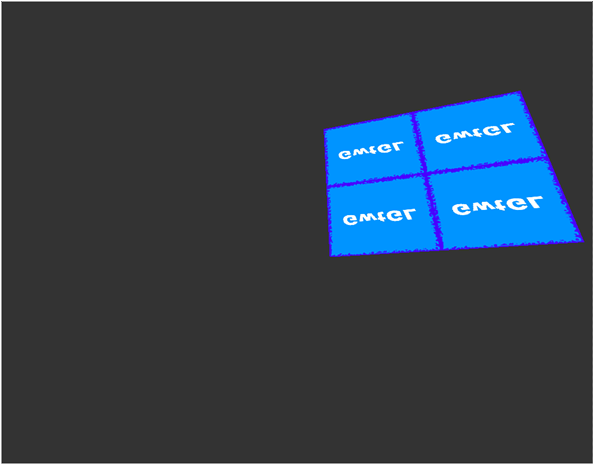
\includegraphics[width=0.5\textwidth]{images/webgl_perf0}}
  \subcaptionbox{Level 2 subdivision}{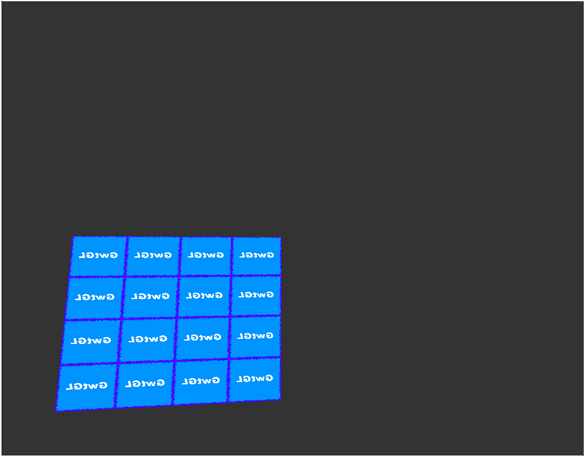
\includegraphics[width=0.5\textwidth]{images/webgl_perf1}} 
  \caption{Illustrating how the subdivision of the quad performance test works}
  \label{fig:webgl_perf}
\end{figure}

\begin{figure}
  \centering
  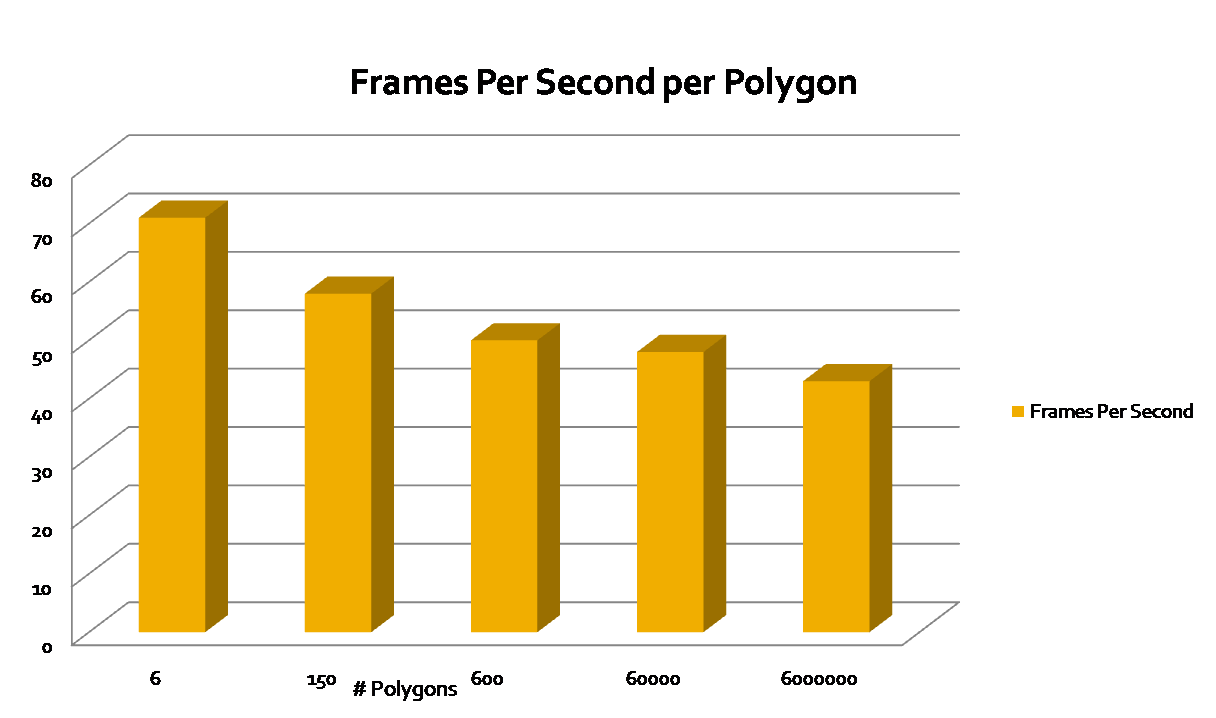
\includegraphics[width=0.8\textwidth]{images/webgl_perf_graph}
  \caption{WebGL framerate as the number of polygons drawn increases. The framerate remains over 40 frames per second, even with 6,000,000 polygons being rendered at once.}
  \label{fig:webgl_perf_graph}
\end{figure}
